\subsection[Wykrywalność (Michał Krakowiak)]{Wykrywalność}
\label{subsec:wykrywalnoscMK}

Windows 10 pokazuje okienko o podłączeniu niezidentyfikowanego urządzenia, chcę tu zrzuty ekranu z narzędzi administracyjnych systemu i wspomnianego komunikatu.
Wykorzystanie możliwości konfiguracji gadżetu USB w czasie wykonywania programu może skutkować chwilową błędną identyfikacją urządzenia przez system operacyjny (w analizowanym przypadki Windows 10). W rezultacie użytkownik zostanie poinformowany stosownym komunikatem ostrzegawczym. Zaawansowany technicznie użytkownik może skorzystać z narzędzi administracyjnych dostarczanych przez system operacyjny w celu zlokalizowania przyczyny komunikatu.
\begin{figure}[H]
    \centering
    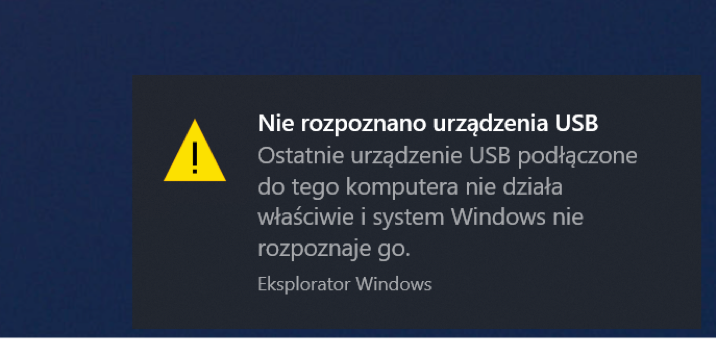
\includegraphics[width=\textwidth]{mk03}
    \caption{Alert}
    \label{fig:windows1}    
\end{figure}
\begin{figure}[H]
    \centering
    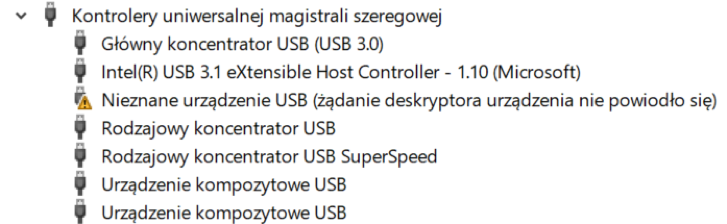
\includegraphics[width=\textwidth]{mk04}
    \caption{Alert2}
    \label{fig:windows2}    
\end{figure}